As previously mentioned, all ideas related to this work were implemented making use of existing technologies. The following sections are dedicated to a brief description of each of them.  

\section{Virtualization}
Virtualization technologies allow running one or more virtual machines, called \emph{guests}, on the same physical server, called \emph{host}. The core idea is to create virtual servers that can run as if they were running on a real physical machine. The entire operating system and its applications can be run inside a virtual machine. Guest systems are completely managed by a software layer running inside the host, which is referred to as the \emph{hypervisor} or \emph{Virtual Machine Monitor} (VMM). The hypervisor is responsible for virtualizing all the physical resources that are assigned to a virtual machine, such as CPUs, memory and I/O devices. Guest virtual machines are typically forced to interact only with the virtualized resources, and the hypervisor itself prevents them to deal with the physical ones. 
\par In general, there are mainly two approaches to implement hypervisors: Type-1 and Type-2 hypervisors. Type-1 hypervisors are also called \emph{bare-metal hypervisors}. They are installed directly on the hardware and have direct access to each physical resource. This can be seen both as an advantage and a disadvantage: direct access to physical resources often allows to obtain better performance, but at the cost of being too hardware dependent, thus reducing portability. On the other hand, Type-2 hypervisors run on top of an operating system: they can access hardware resources only through the usage of the underlying operating system, exploiting the portability of the operating system itself and its drivers, at the cost of slightly degrading the performance of virtual machines. However, sometimes the distinction between Type-1 and Type-2 hypervisor is not so clear. In this work, the KVM hypervisor is used: it can be considered as a mix of the two approaches since it makes use of hardware virtualization features directly as if it was a Type-1 hypervisor, but at the same time tries to reuse many of the features of the Linux kernel for its own purposes, as in Type-2 hypervisors. More details on it are in the following sections. 
\par The virtualization problem has been faced in many ways, leading to as many ways of implementing it. In particular, there exist at least three main different solutions to the problem.
\subsection{Emulation} \label{sec:emul}
The first one is the so-called \emph{emulation}. An emulator is a program that is typically built around a main loop. Its purpose is to mimic the actions that would be performed by the target machine processor, such as fetching, decoding and executing instructions. Typically, it is possible to think about the execution phase of the processor as a big switch, having one case for each possible instruction belonging to the instruction set of the target machine. Each of those instructions is then translated into actions, i.e host instructions, performed by the hypervisor, allowing for the possibility to run any software that was originally written for another machine, potentially with a different architecture and instruction set w.r.t the host. Usually, emulators are implemented as userspace programs in the host system and they are in charge of virtualizing every resource used by the guest. To do that, a different data structure for each of the resources available to the guest is used. For the sake of clarity, it is possible to think about the simplest machine as if it was made up of only its CPU and memory. Then, the CPU can be defined as a collection of registers and memory as an array of bytes, allocated in the virtual address space of the process running the emulator. When executing instructions, the emulator will modify the state of these resources according to their semantic. Of course, when it comes to emulating a much more complex machine, many other features have to be taken into account, such as interrupts and I/O devices, but in general the approach to be used is the same for any hardware resource. Also, it has to be noted that the emulator can make use of all the functionalities offered by the host operating system to implement any kind of hardware resource. For instance, considering a virtual disk used by the virtual machine to store data, it can be easily implemented using a file in the host. The disk will be accessed by the target processor instructions related to I/O and the emulator can implement those instructions using filesystem-related system calls, such as \emph{open}, \emph{read}, \emph{write} and \emph{close}. On the other hand, however, introducing I/O devices is also one of the biggest challenges in emulation. This is because I/O devices often perform operations asynchronously w.r.t to the main loop implementing the CPU. Typically, this problem is solved by using multithreading, assigning one thread to the CPU and one or more threads to I/O devices. This may introduce race conditions and interference problems within the emulator, thus all objects that need to be accessed by multiple threads must be protected using synchronization techniques, increasing the complexity of the emulator itself.
\par The emulation approach can be considered as a naive approach to virtualization. The emulator is simply scanning guest instructions one by one and translating them into pieces of software running on the host. It is often the case that one guest instruction is translated into many host instructions, leading to a non-negligible overhead. Techniques like binary translation aim at improving the performance of emulation by translating blocks of guest instructions into host instructions. By looking at many instructions at a time, it is possible to optimize, for instance, the number of host instructions needed. Furthermore, binary translation often caches translated blocks to reuse them when the same guest block is hit again. However, even this approach cannot reach near-native performance and thus other approaches to virtualization were introduced to let virtual machines run much faster. Finally, even if this is not the approach used in data centers, it has some concepts that are to some extent reused in other approaches and that are useful for the purposes of this work. 

\subsection{Trap \& Emulate}
Trap \& Emulate approach tries to overcome the limitations of emulation. The fundamental idea behind this approach was to try to run virtual machines having the same architecture and instruction set of the host as low privileged userspace processes. Anytime a VM is executing, the CPU directly takes orders from the guest. This is possible only because the instruction set of the guest is exactly the same as the one of the host. Of course, there is the need to put limitations on what the guest system can do. Those limitations are introduced by the fact that the virtual machine is running with low privileges: anytime the guest operating system tries to execute a privileged instruction, a trap will be generated. Through this trap, the hypervisor can regain control of execution, taking care of correctly emulating the instruction that caused the trap on behalf of the guest, thus limiting what the guest virtual machine can do. For instance, think about the \texttt{IN} and \texttt{OUT} instructions on x86 architectures. As these are privileged instructions, all I/O operations will be handled by the hypervisor, preventing the guest to execute operations on real hardware. However, this approach was not completely feasible on some architectures, in particular x86 architectures. This is because the instruction set contains instructions that behave differently if executed at different privilege levels. In particular, those instructions will not trap, leading to inability of the hypervisor to regain control of the execution, even if that instruction should have been emulated. Most of those instructions are related to memory management and interrupt handling, but their discussion is out of the scope of this work. Anyway, the Trap \& Emulate can be considered as the main starting point for all modern techniques used nowadays.

\subsection{Paravirtualization}
Paravirtualization is one of the proposed solutions to alleviate the problem of not being able to trap all the desired instructions, specifically on x86 architectures. This problem mainly arises because one of the requirements that was implicitly taken into account was to run unmodified versions of the guest operating system. Paravirtualization releases this constraint and tries to make the guest operating system aware that is being virtualized and able to communicate with the hypervisor. This is accomplished by replacing all instructions which are hard to virtualize with \emph{hypercalls}. The hypercall notion is very similar to the one of system calls: as system calls are used to let userspace processes communicate with the operating system, hypercalls are used to let guest virtual machines communicate with the hypervisor. With hypercalls the hypervisor can easily regain control of the execution every time it is needed and emulate those that were difficult-to-virtualize instructions. 
\par This is how paravirtualization solves the problem of the Trap \& Emulate approach. However, it introduces many other problems. In fact, paravirtualized systems fully rely on the interface exposed by the hypervisor. If that interface changes, they are not able to run, thus portability is drastically reduced. Furthermore, it may be difficult or impossible  to have support for closed source operating systems.
Other techniques like hardware-assisted approaches virtualization in a different way and without any guest modifications, as it is explained in the following, but the idea of hypercall is essential to the purpose of this thesis and it will be recycled in the proposed system. 

\subsection{Hardware-assisted virtualization}
Another way to solve the problems related to the Trap \& Emulate approach is hardware-assisted virtualization. This kind of approach is based on a simple consideration: while the virtual machine is running and giving orders directly to the CPU \footnote{the same ISA case is considered again}, the only way to restrict the actions of the guest is by means of the hardware. In recent years, both Intel and AMD added virtualization features to their processors, which aim at offering support to hypervisors. In the following, only Intel's ones will be considered, which are grouped into Intel Virtualization Technology. In general, hardware is modified to specifically and selectively put controls on guest systems. This can be done if the hardware itself is aware of whether it is a virtual machine or the hypervisor that is running. To determine these two states, a simple bit can be used. This idea led to the introduction of the \emph{root} and \emph{non-root} mode in Intel processors. When the processor is in root mode, the hypervisor is executing and the VM is on pause. Contrarily, when a VM is executing, the processor is in non-root mode. It is worthwhile noticing that these two new states of the processor are completely \emph{orthogonal} to the already existing system and user mode (Ring 0 and Ring 3 in protected mode), leading to four different combinations: \emph{root/system, root/user, non-root/system} and \emph{non-root/user}, which are typically associated with the host OS, host applications, guest OS and guest applications, respectively, as also shown in Figure \ref{fig:intel-vt}. Thanks to the introduction of this new mode of operation, guest systems can now switch between userspace and kernel space without hypervisor intervention, something that was impossible using the Trap \& Emulate approach. 
\begin{figure}
    \centering
    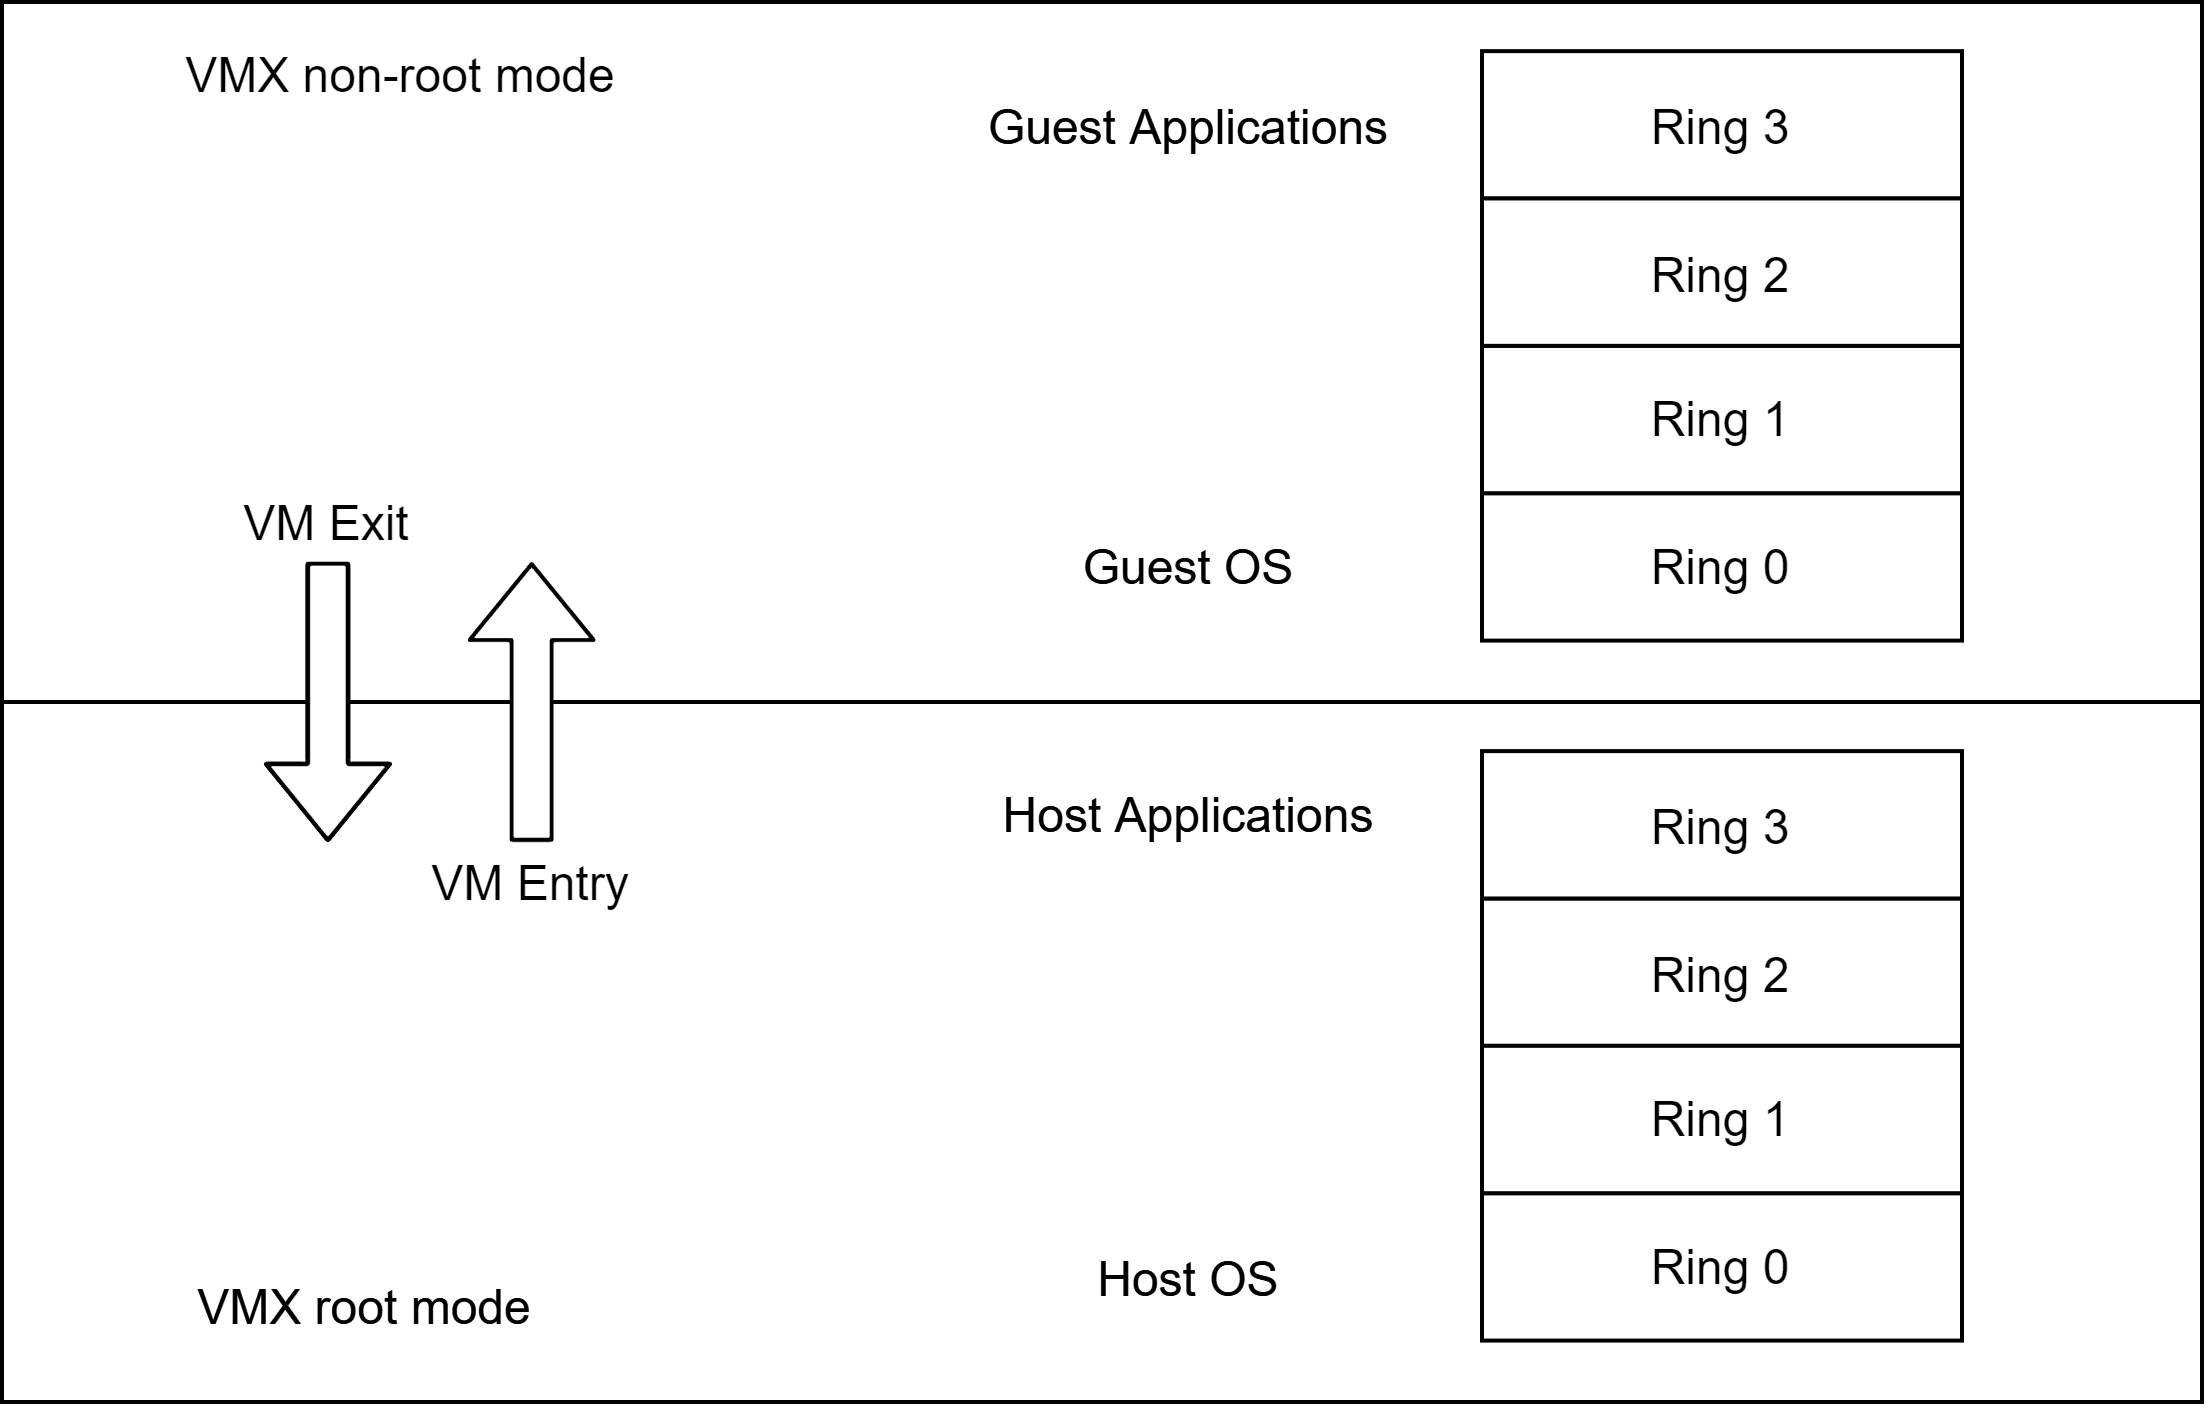
\includegraphics{images/root-nonroot.png}
    \caption{Representation of Intel Virtualization Technology}
    \label{fig:intel-vt}
\end{figure}
\par
Whenever the guest kernel tries to execute an instruction that needs the intervention of the hypervisor, the hardware forces a transition from non-root to root mode, letting the hypervisor regain control of execution. This event is defined as \texttt{VM EXIT}. On \texttt{VM EXIT}, the hardware also takes care to let the hypervisor know the \emph{exit reason} of the VM. This information can be used to correctly emulate the instruction that caused the exit on behalf of the guest. After the emulation of such instruction, the hypervisor turns the processor into non-root mode and starts the VM again, which will continue its execution with the instruction next to the one that caused the exit. To handle this mechanism, Intel has designed and implemented new instructions and defined new data structures. First, since this is a new feature of Intel processors, hypervisors can discover support for Intel Virtualization Technology by executing the \texttt{CPUID} instruction. This instruction returns processor identification and feature information to the \texttt{EAX}, \texttt{EBX}, \texttt{ECX} and \texttt{EDX} registers. If bit 5 in \texttt{ECX} is set, it means that the processor supports Virtual Machine Extensions (VMX), meaning that hardware-assisted virtualization is possible. To enter and exit VMX operation mode it is possible to use the \texttt{VMXON} and \texttt{VMXOFF} instructions. When VMX is turned on, the hypervisor can make use of all the other newly introduced instructions. In particular, transitions from root to non-root mode are achieved by means of \texttt{VMLAUNCH} and \texttt{VMRESUME}, used to start and resume virtual machines.
\par
Many of the VMX instructions are related to the handling of the Virtual Machine Control Structure (VMCS). This is one of the most important data structures used to implement the mechanisms briefly introduced before and it is worthwhile being aware of its detail in depth. This data structure is used to manage VM entries and VM exits and to define the processor behavior in non-root mode. It can be manipulated by means of the new instructions \texttt{VMCLEAR}, \texttt{VMPTRLD}, \texttt{VMREAD} and  \texttt{VMWRITE}. The hypervisor maintains several VMCSs, typically one for each processor of each virtual machine. Out of all the VMCSs, only one can be the current VMCS and that one is pointed by a specific processor register. To make current a specific VMCS, the instruction \texttt{VMPTRLD} can be used. All instructions used to manipulate the VMCS have effects only on the current VMCS. Usually, hypervisors reserve 4KB to store VMCSs, which are organized into six logical groups:
\begin{itemize}
    \item Guest-state area. The state of the guest processor is stored and loaded using this area on \texttt{VM EXIT} and \texttt{VM ENTRY}, respectively. The processor is of course saved by using the set of its registers, including its general-purpose registers, control registers, debug registers and so on. The value stored in the instruction pointer can be used to determine the instruction that caused the \texttt{VM EXIT} and to locate the first instruction that the guest should execute on \texttt{VM ENTRY}.
    \item Host-state area. This area is used to load the state of the host processor on \texttt{VM EXIT}. All the host's registers are saved in this area on \texttt{VM ENTRY}. Since the entire state of the host processor is saved here, the guest can freely modify its own registers without affecting the host.
    \item VM-Execution control fields. This area defines controls on the processor behavior which are put in place when in non-root mode. They determine in part the causes of \texttt{VM EXIT}. These fields are used to specify what should happen both on asynchronous events (e.g. interrupts) and synchronous events. For the latter, two 32-bit vectors are used to determine which events or instructions should cause a \texttt{VM EXIT}. Examples of these controls are CR3-load and CR3-store exiting, enabling second level address translation (Extended Page Tables in Intel), Descriptor-table exiting (exiting on LIDT or SIDT execution) and many others.
    \item \texttt{VM EXIT} control fields, used to control \texttt{VM EXIT}.
    \item \texttt{VM ENTRY} control fields, used to control \texttt{VM ENTRY}.
    \item \texttt{VM EXIT} information fields. This area contains data related to the reason that caused the last \texttt{VM EXIT}. It is used to understand what has happened and what the hypervisor should do before entering in non-root mode again.
\end{itemize}
\par
Another important feature offered by Intel Virtualization Technology is hardware support for the virtualization of the guest Memory Management Unit (MMU). The introduction of this new feature heavily improved older implementations of virtualization of virtual memory, such as shadow page tables. In general, the task of MMU virtualization involves translating Guest Virtual Addresses (GVA) into Host Virtual Addresses (HPA). The guest kernel is only able to prepare mappings to perform the translation from GVA to Guest Physical Addresses (GPA), maintaining its own page tables. To go further in the translation and to put controls on the memory accessed by the guest, it is clear that the hypervisor should be involved in some way. When using the shadow page tables approach, hardware will never use the guest page tables directly. Instead, the hypervisor forces a \texttt{VM EXIT} whenever the guest tries to modify the CR3 register or its own page tables and performs actions to let the guest access memory only where it is supposed to, by using host page tables. In this way, guest will use the mappings prepared by the hypervisor and the MMU will continuously perform translation from GVA directly to HPA. This is a completely working approach, but it is very expensive: \texttt{VM EXIT}s involves very time-consuming operations, such as saving the guest's state and loading the host's one, examining the exit reason, and perform operations accordingly. For this reason, the number of exits should be maintained as low as possible, otherwise, virtual machines will have to pay a great performance overhead.
\par 
To overcome these issues, Intel implemented a second-level address translation approach, Extended Page Tables (EPT) in their jargon. The idea behind this approach is simple: the host processor, and specifically the host MMU, is capable of holding two pointers. The translation of a guest virtual address starts by using the guest's CR3 register, which is loaded in the physical CR3 register when the VM is running. Through the usage of its CR3 register, the VM is able to translate any guest virtual address to guest physical address. Then, each guest's physical address needs to be translated into its corresponding host physical address, and this is done with second-level page tables, which are completely managed by the hypervisor and equivalent to the normal page tables. To maintain these second-level page tables, the MMU is equipped with the second pointer, called \texttt{EPTP}. Hardware uses these second-level page tables when the processor is in non-root mode. The guest can now modify its own page tables without neither hypervisor intervention nor \texttt{VM EXIT}s since the translation now happens in hardware and second-level page tables are prepared by the hypervisor, solving the performance problems of the previous approach. It must be noted, though, that the overhead is paid in another way: a translation of a guest's virtual address now involves up to 24 memory accesses, assuming four-level page tables both for the guest and the host. This can be explained by following all the steps involved in the translation:

\begin{itemize}
    \item First, the translation of a GVA must start from the guest CR3. This register contains a GPA, which in turn must be translated before actually accessing the guest level-4 table. The translation of the address in CR3 requires a walk in the second-level page tables of the host, thus four memory accesses. Then, after the translation of CR3, it is possible to access the guest level-4 table with one more memory access, resulting in five memory accesses.
    \item After gaining access to level-4, a part of the GVA is used to index that table to access the corresponding level-3 table. Again, the pointer to this table is a GPA that must be translated too. Four accesses are needed for the translation and one more access for the level-3 table. 
    \item The previous steps must be performed also for level-2 and level-1.
    \item In the last step, the translation is retrieved. The obtained GPA corresponding to the translation of the initial GVA has to be translated again into a HPA, and this adds just four memory accesses, resulting in 24 accesses in total before accessing the needed data.
\end{itemize}
\begin{figure}[t]
    \centering
    %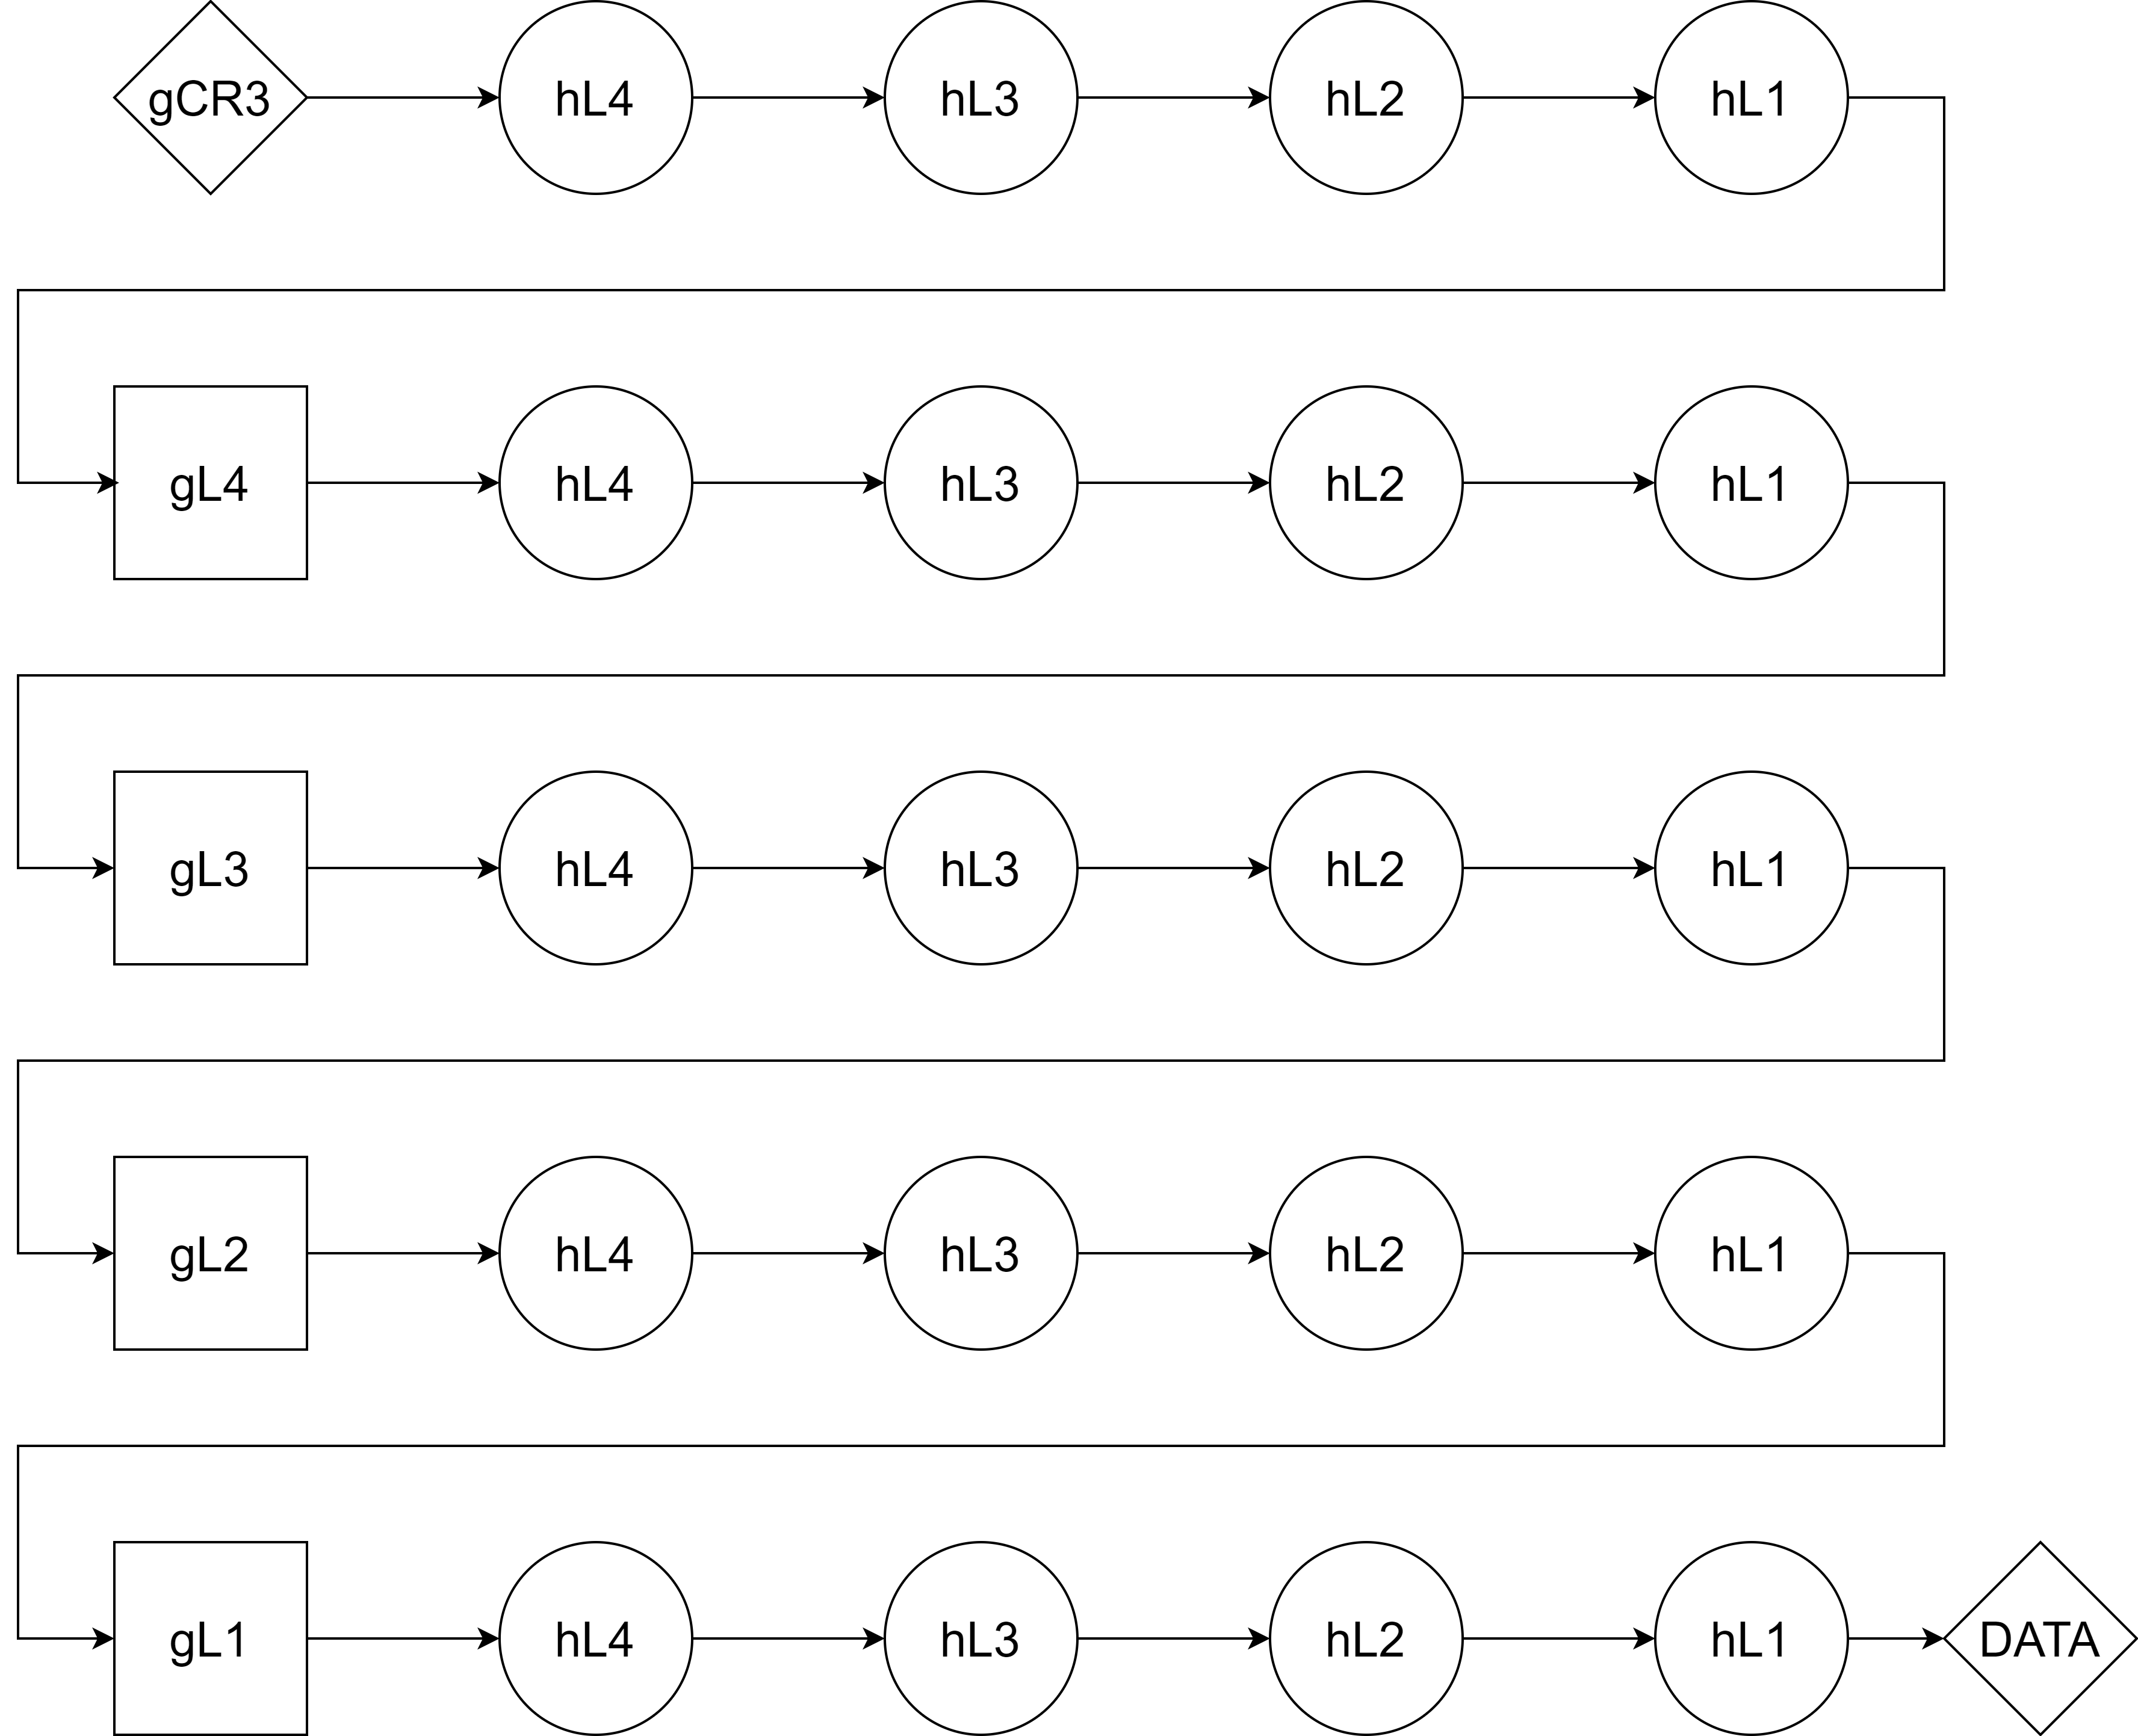
\includegraphics[width=\textwidth]{images/two-dimensional-walk.png}
    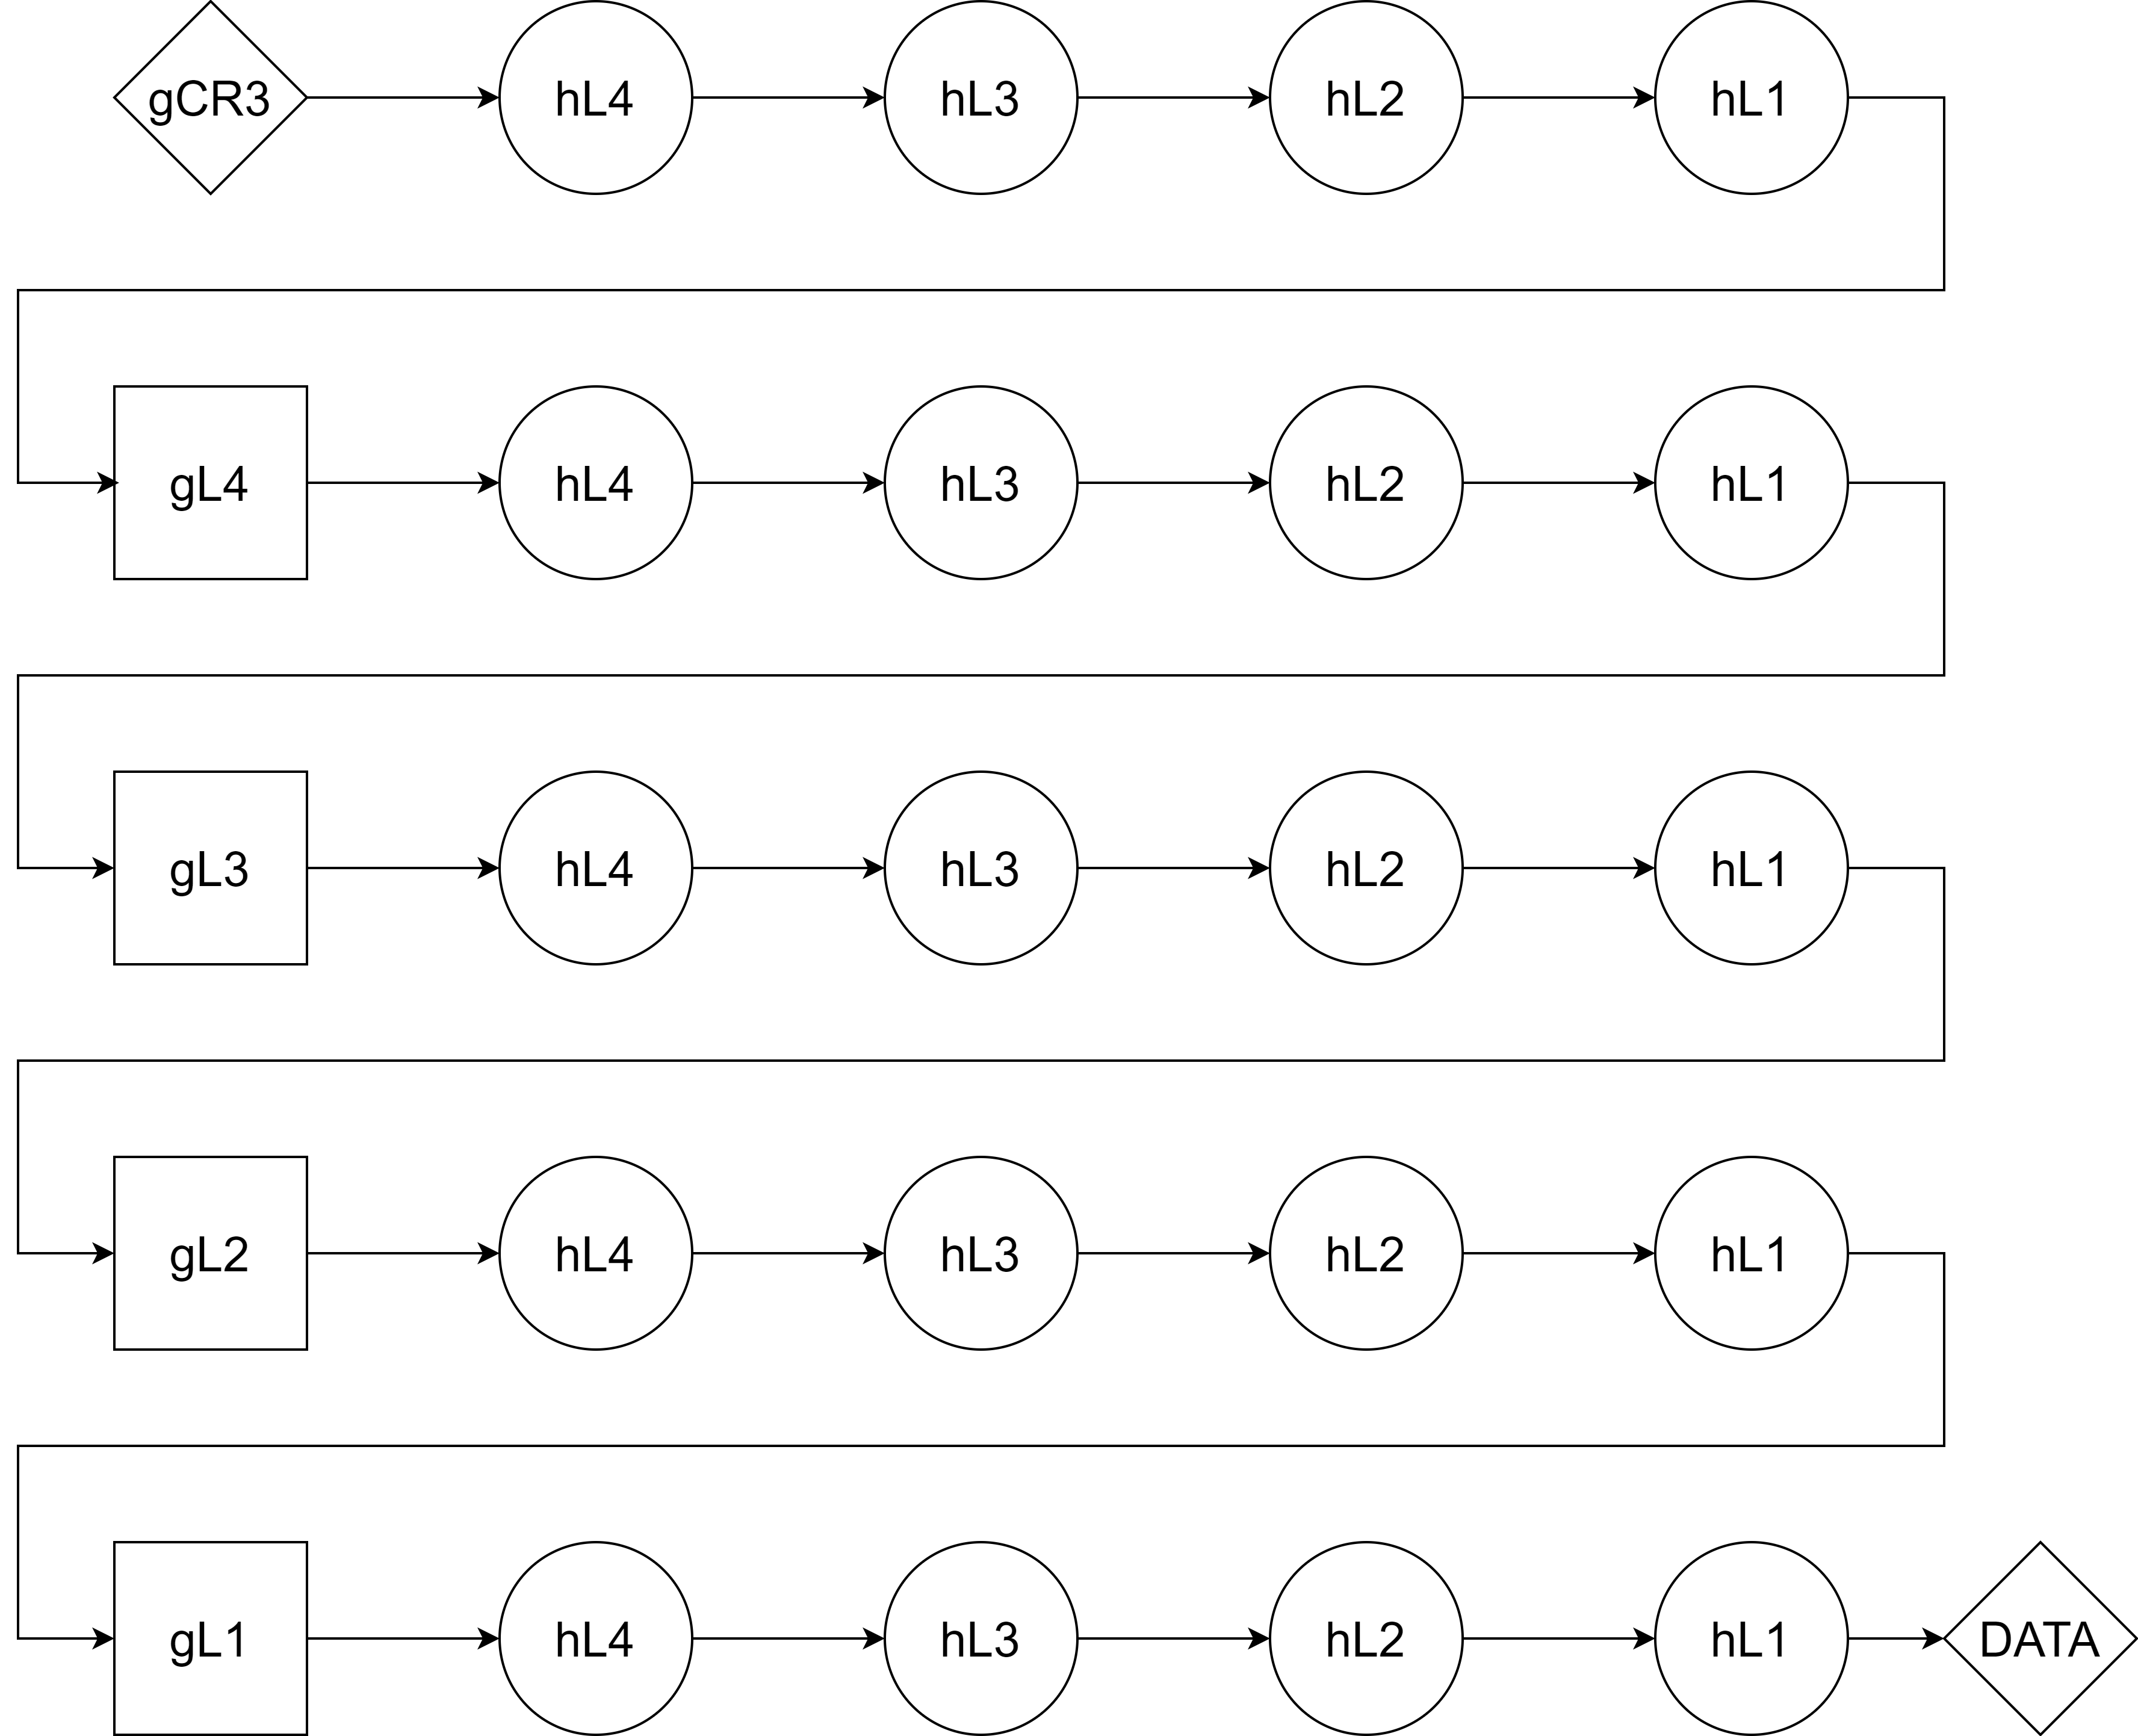
\includegraphics[scale=0.6]{images/two-dimensional-walk.png}
    \caption{The two-dimensional page table walk. Host page tables are walked horizontally, while guest's ones are scanned vertically, resulting in 24 memory accesses before accessing data.}
    \label{fig:intel-ept-translation}

\end{figure}
For the sake of clarity, Figure \ref{fig:intel-ept-translation} shows the steps just discussed. The result of these steps is a 2D page walk, both in the host and guest directions, and that is the reason why this approach is also called Two Dimensional Paging. To avoid performing these long page table walks, the processor is equipped with many TLBs to cache the recently used translations. Furthermore, another way to decrease the number of memory accesses in case of a TLB miss is using bigger-sized pages, to shorten the length of the walk. 
\par 
This is the most widely adopted approach to MMU virtualization today since it outperforms many of the previous ones, shadow page tables included. Another important aspect of the second level page tables is that both table and page descriptors have their own control bits: in fact, the hypervisor can use these bits to enforce a specific kind of memory access, such as read, write or execute access, or combinations of them. Furthermore, through the usage of the access and dirty bit, it can understand which pages were accessed, written, and, by consequence, read. To use these bits, however, the hypervisor must know which are the memory areas requiring such protections and with which access mode. 


\section{QEMU and KVM}
As mentioned before, hardware-assisted virtualization offers support for implementing hypervisors. Kernel-based Virtual Machine (KVM) \cite{kvm} is a Linux subsystem developed to transform Linux into a hypervisor, leveraging the newly added features for virtualization. On the other hand, QEMU is an emulator and it can be used to run target systems with a different architecture with respect to the host, or when the guest's and host's architecture are the same, it can make use of KVM by setting up virtual machines using its API. In this way, QEMU can leverage KVM for creating and managing virtual machines, adding memory and CPUs to them. Then, it has also the responsibility for emulating virtual devices attached to them, such as keyboards, hard drives, PCI devices, and network cards. This is always done in the same way by QEMU, both when it works as a hardware emulator and when it uses KVM with hardware-assisted virtualization.
\par 
Both QEMU and KVM are open source software and they are a perfect fit for this work. The source code is readily available on the Internet and it can be studied and modified for different purposes, like the ones discussed here. This work tries to modify the part of QEMU's code using the KVM API and the KVM kernel module itself to achieve its goals, thus it is worthwhile explaining the high-level architecture of both. 
\par 
KVM is structured as a Linux character device. Its device node is \texttt{/dev/kvm} and it can be used from userspace, e.g from QEMU, through a set of \texttt{ioctl} system calls. Typical operations that can be issued are:
\begin{itemize}
    \item Creation of a new virtual machine
    \item Allocation of memory to a virtual machine 
    \item Reading and writing virtual CPU registers
    \item Running a virtual machine
\end{itemize}
\begin{figure}[t]
  \centering
  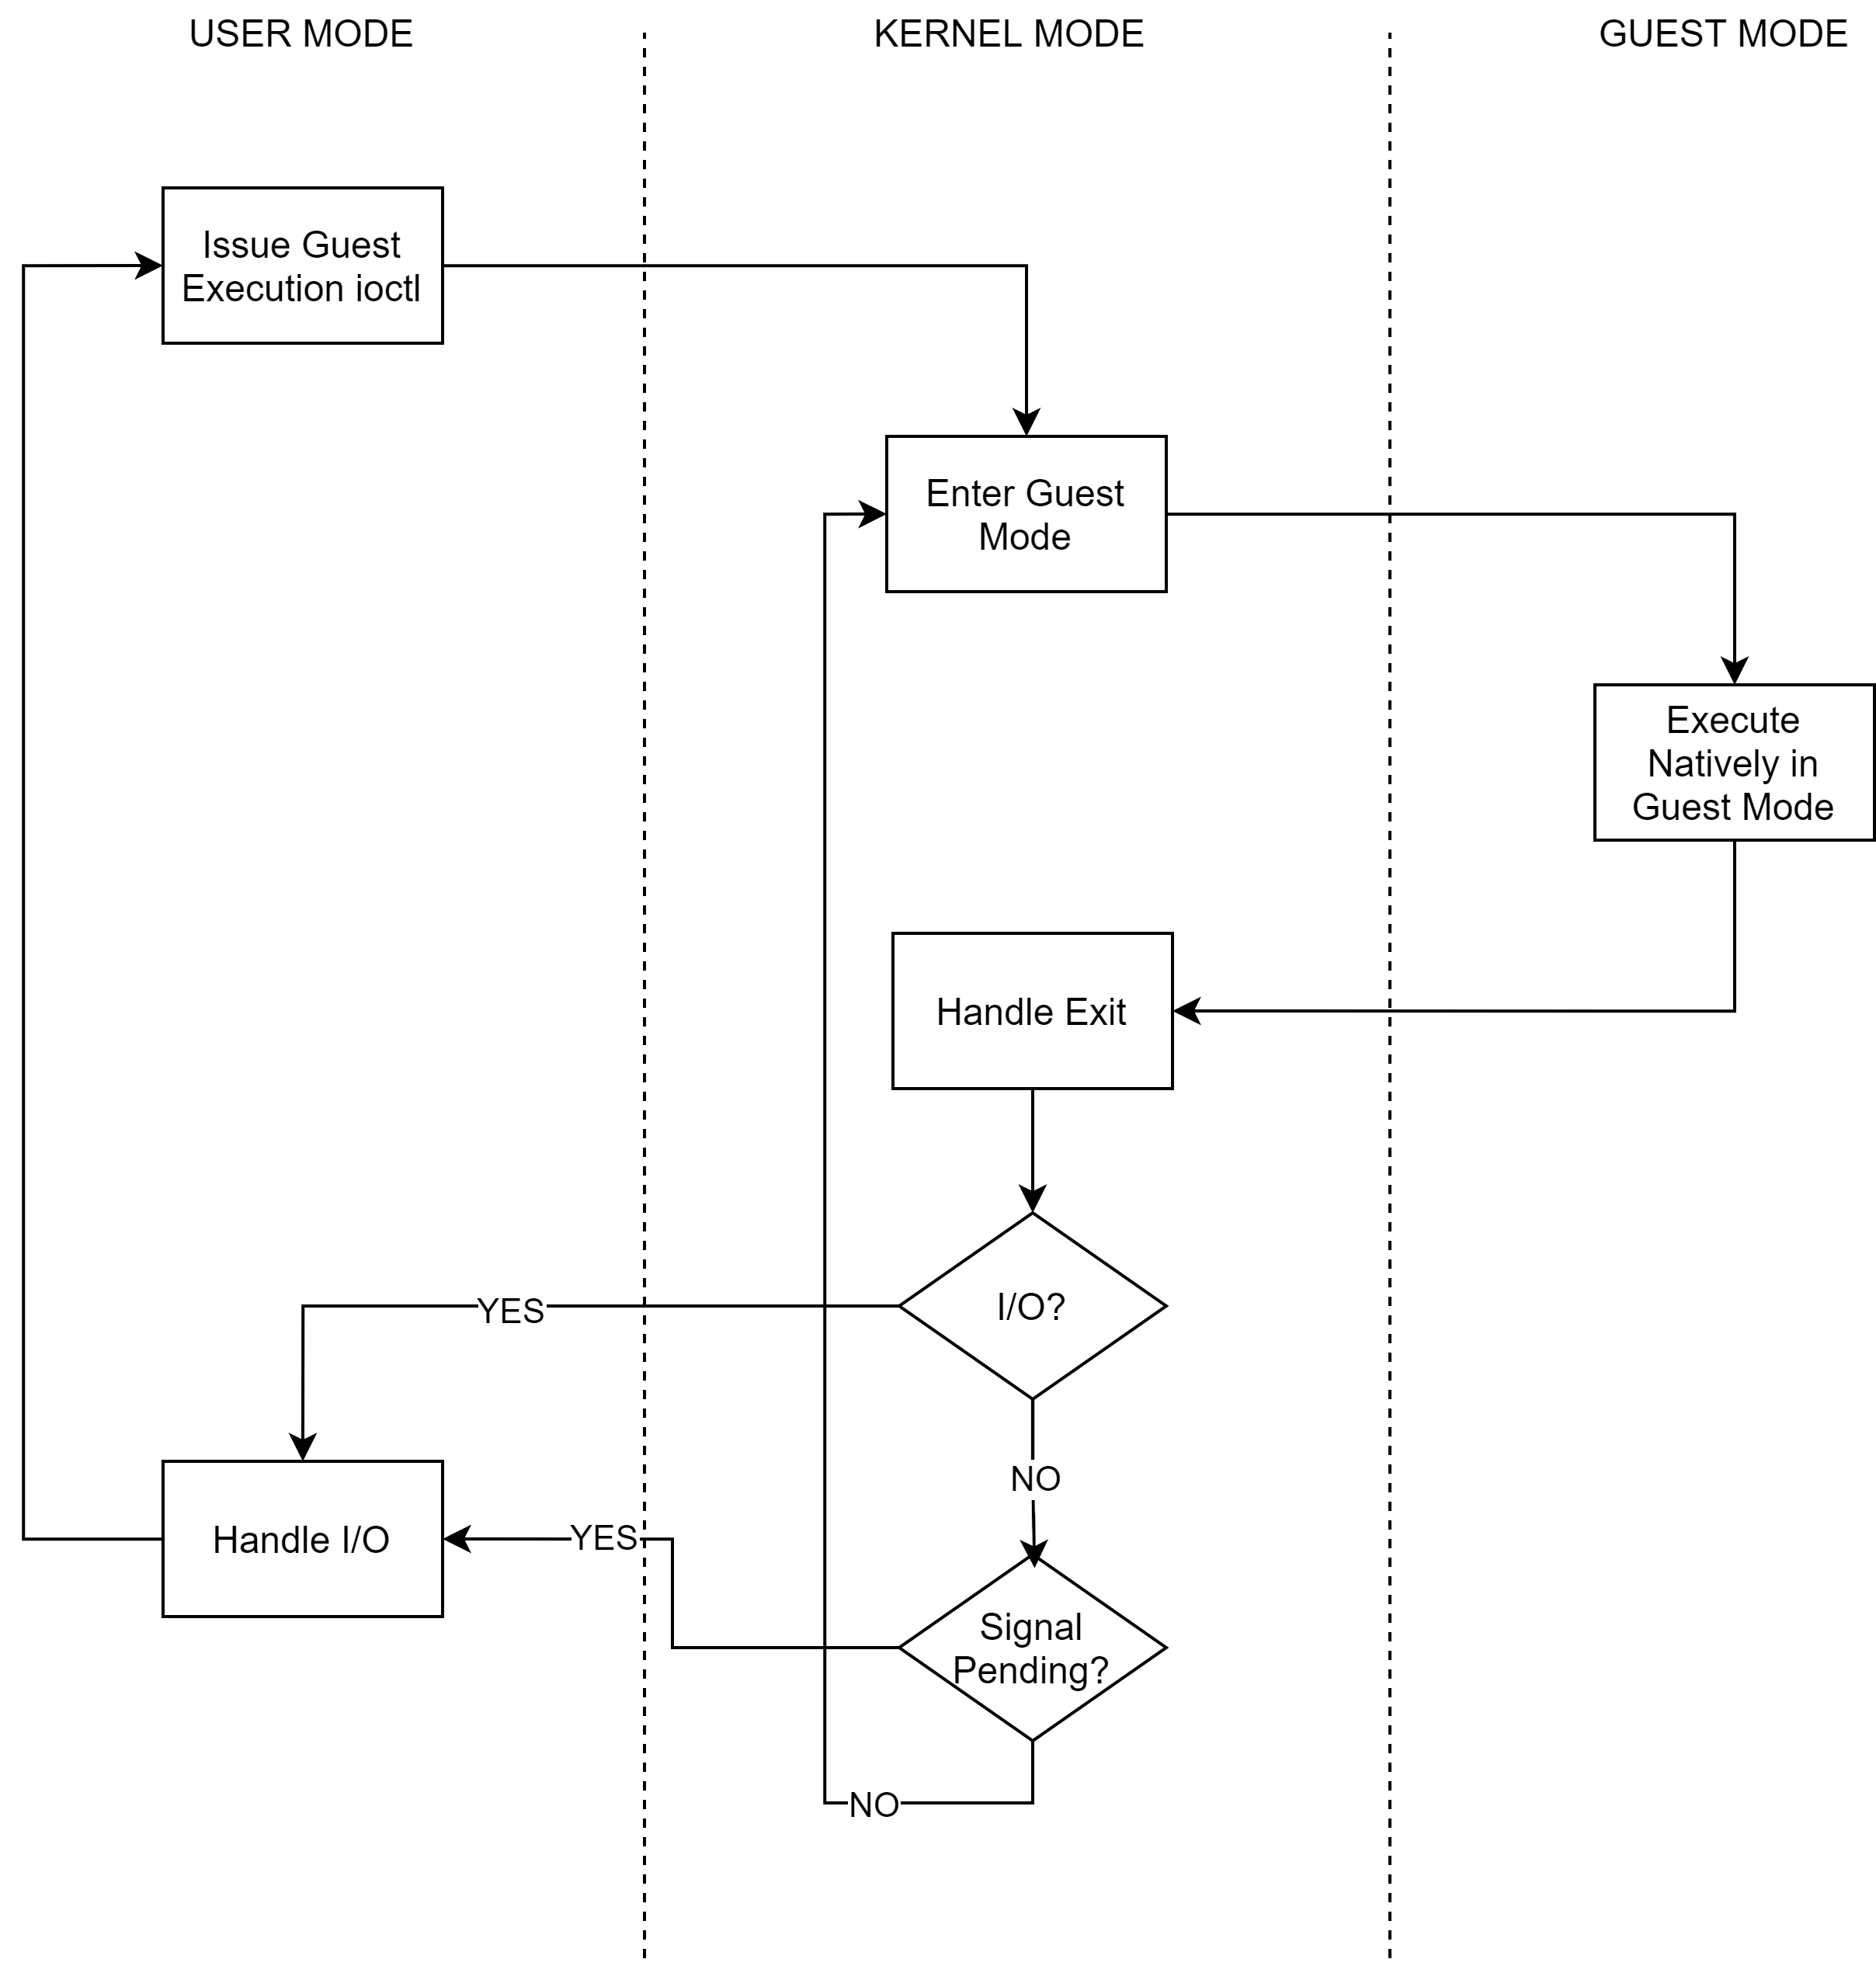
\includegraphics[scale=0.80]{images/kvm-guest-execution.png}
  \caption{KVM guest execution loop}
  \label{fig:kvmloop}
\end{figure}
\par
Once the virtual machine is configured (e.g, the userspace process corresponding to QEMU has attached memory and CPUs to the VM through the usage of the KVM API), the guest gets executed in a triply nested loop, as shown in Figure \ref{fig:kvmloop}. 
The userspace process asks the kernel to execute the virtual machine, thanks to the \texttt{KVM\_RUN} ioctl. The kernel performs the actions needed to execute the guest. In particular, in Intel architectures, it will execute a VMLaunch instruction once the corresponding VMCS is correctly set up, forcing the processor to enter the non-root mode. After this step, the guest is executed until a VMExit occurs. If the exit reason is related to an I/O instruction, for instance, it will be completely handled in userspace and, in this case, in the QEMU process. Once QEMU has emulated the instruction, it will issue again the ioctl to run the virtual machine and so on. This is the most simple way to explain how QEMU and KVM cooperate to implement a complete hypervisor. 

\subsection{QEMU threading model}
To deeply understand how QEMU works, it is fundamental to be aware of its threading model, which is thoroughly depicted in Figure \ref{fig:qemu}. As already mentioned, QEMU is a userspace event-driven multithreaded application. The entire QEMU process is used to model the whole virtual machine. When using QEMU with KVM enabled, its main purpose is to virtualize I/O and interact with the KVM kernel modules for guest code execution. In particular, the part of QEMU regarding I/O is strongly based on events. In fact, QEMU makes use of the I/O thread to let the virtual machine interact with the external world. The I/O thread is centered around a big main loop that makes use of the \texttt{select} or the \texttt{poll} family of system calls, waiting for new file descriptors to become ready. Whenever a file descriptor is ready, the main loop is responsible for \emph{reacting} to this event by calling the corresponding \emph{callback} function. This behavior can be fully summarized using the \texttt{qemu\_set\_fd\_handler} function as an example: it allows to add a file descriptor to be monitored by the main loop. File descriptors typically become ready for read and write operations, and that is why the previous function takes as an argument both a read and write callback. Using this logic, file descriptors callbacks will execute sequentially one after the other and in a non-blocking fashion since callbacks will invoke I/O functions only on ready file descriptors.

\begin{figure}[t]
    \centering
    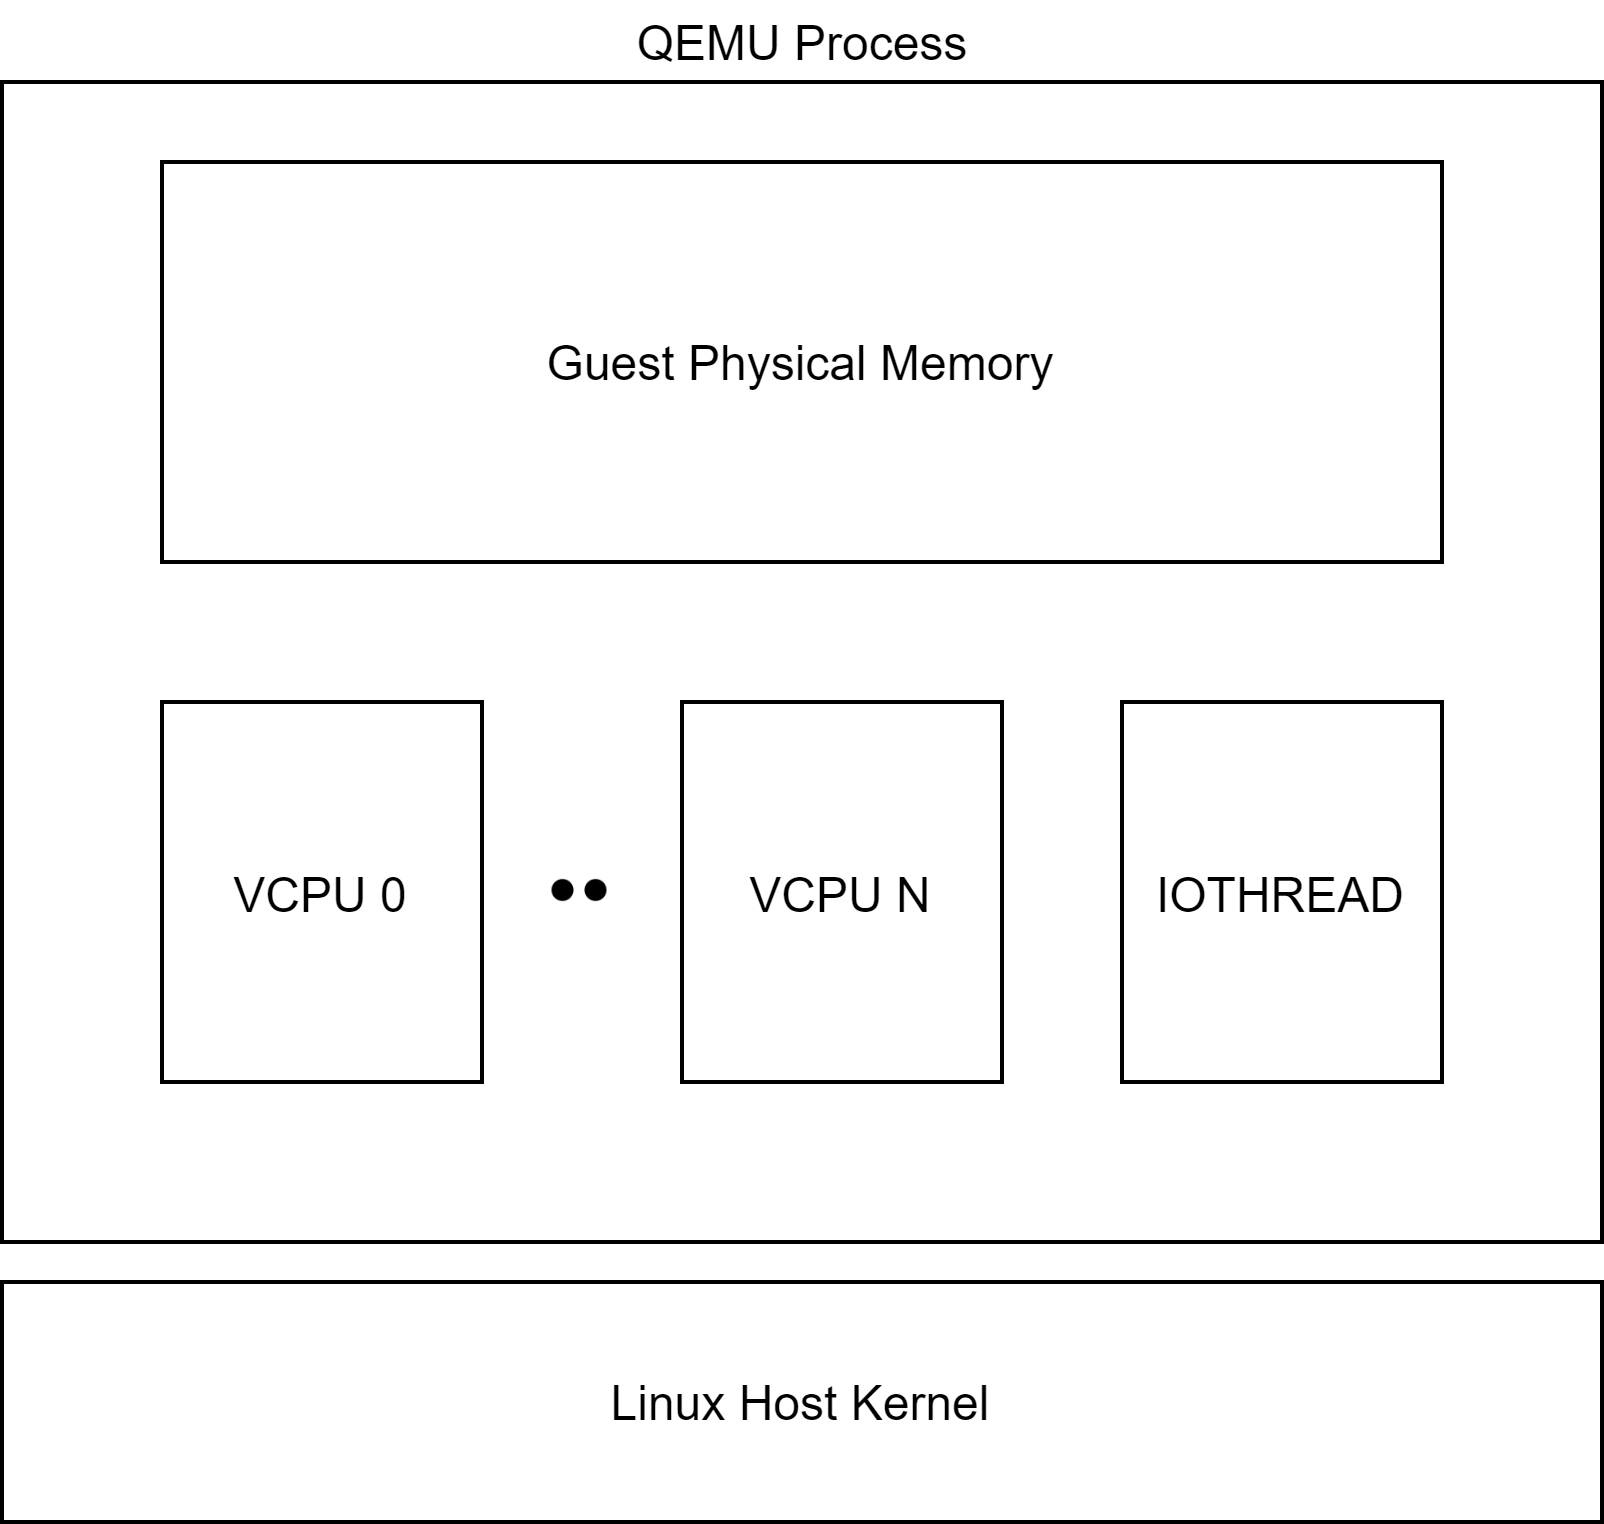
\includegraphics{images/qemu.png}
    \caption{QEMU threading model}
    \label{fig:qemu}
\end{figure}

\par 
Another important aspect regards the execution of the guest code itself. Each virtual CPU attached to the VM corresponds to a thread inside QEMU. These threads are responsible for executing the loop shown in the already discussed Figure \ref{fig:kvmloop}. It has to be noted that the vCPU thread continuously switches between guest execution and handling of I/O events. Thus, it is clear that data structures representing I/O devices are accessed concurrently both by vCPU and I/O thread, as already discussed in Section \ref{sec:emul}. In particular, it can be noticed how the emulation approach and the one discussed are pretty similar. The only difference consists in the way guest code is executed: in the emulation approach, guest instructions were executed through the use of the execution loop, while in this approach guest instructions are directly executed on the CPU, using all the features of hardware-assisted virtualization. Furthermore, since vCPUs are modeled as threads, they are scheduled as normal threads in the system and the QEMU process can make use of signals whenever it wants to stop the execution of the guest. 

\subsection{KVM kernel modules}
The proposed solution will also try to modify the KVM kernel modules to accomplish its goals, and that is why it is relevant to briefly discuss how it is organized internally. 
\par 
KVM is organized in two kernel modules: one is the \texttt{kvm.ko} and the other is architecture-specific. Since the Intel VT-x technology is being used, the \texttt{kvm-intel.ko} modules will be used. Specifically, the first module will detect the type of processor of the machine and will load the needed module accordingly. The two main files of KVM are \texttt{kvm-main.c} for the generic part of KVM and \texttt{vmx.c} for the Intel specific part. 
\par 
The \texttt{/dev/kvm} character device is implemented as a \texttt{misc\_device} and it is possible to let the kernel handle the ioctls by associating to it the appropriate \texttt{file\_operation} struct, as reported in Listing \ref{list:kvm-char}.

\begin{lstlisting}[style=c, caption={KVM character device}, label={list:kvm-char}]
static struct file_operations kvm_chardev_ops = {
	.unlocked_ioctl = kvm_dev_ioctl,
	.llseek		= noop_llseek,
	KVM_COMPAT(kvm_dev_ioctl),
};

static struct miscdevice kvm_dev = {
	KVM_MINOR,
	"kvm",
	&kvm_chardev_ops,
};
\end{lstlisting}
The userspace part will also deal with other file descriptors such as the VM and VCPU file descriptors. The latter two are installed in the file descriptor table of the process by means of anonymous inodes, since there are no files or character devices that are backing them. In any case, it is possible to associate a \texttt{file\_operation} struct pretty much in the same way, using the \texttt{anon\_inode\_getfile} function. The functions that are supposed to be called and respond to ioctls are organized in big switches, having one statement for each possible ioctl. 
\par
From the point of view of KVM, a virtual machine is completely described by the \texttt{kvm} struct, as reported in Listing \ref{list:kvm-struct}.

\begin{lstlisting}[style=c, caption={Relevant fields of struct \texttt{kvm}}, label={list:kvm-struct}]
struct kvm { 

	...

	struct kvm_memslots __rcu *memslots[KVM_ADDRESS_SPACE_NUM];
	struct kvm_vcpu *vcpus[KVM_MAX_VCPUS];
	
	...
	
	struct kvm_arch arch;
	
	...
	
}

\end{lstlisting}
As it can be noticed, this data structure contains an array of pointers to \texttt{kvm\_vcpu} structs, which is the data structure describing the virtual CPUs. Furthermore, it contains pointers to \texttt{kvm\_memslots} struct which in turn is used to retrieve all the \texttt{kvm\_memory\_slot} structs associated with the virtual machine. More details on how memory is allocated are described in the following, but until now it is sufficient to notice that the set of \texttt{kvm\_memory\_slot}s are used to describe the physical memory of the guest. Lastly, all architecture-dependent features are always encapsulated in a dedicated data structure, such as the \texttt{kvm\_arch} or the \texttt{kvm\_vcpu\_arch} data structures.
\par 
This was a brief description of how KVM is organized internally and will be useful when modifying it to accomplish the objectives of this work. 

\section{Threat modeling}
When it comes to building a system for security, it is important to state the relevant assumptions beforehand. In this work, the attacker is modeled as an external one. Typically, virtual machines are used to offer some services to the external world and they have to be accessible in a certain way. It is assumed that the attacker is able to attack the system from the outside and to escalate its privileges gaining Ring 0 access, with the intention of gaining \emph{persistence} as the last step of the attack. Ring 0 access means that the attacker has the ability to arbitrary read and write in the kernel address space. The final objective of the intruder, i.e persistence of the attack, will let her take full control of the virtual machine anytime. What it is important to underline is that this kind of attack scenario is made up of different steps. A system to protect against it can thus be organized in multiple lines of defense and try to mitigate or even eliminate the risk of being attacked or to do the next step, as the proposed system tries to do. Additionally, awareness on how the attacker can gain persistence is crucial. Attackers often achieved this by means of rootkits, which are installed upon successful attacks.
\par Rootkits are a specific kind of malware that is able to modify the behavior of a running operating system, letting the attacker being able to regain easy access to the root user once the malware is installed. Another rootkit's goal is to hide the fact that the system has been compromised. This is typically done by hiding files, processes, network connections, and so on, so that the attacker's activities are as invisible as possible. Since rootkits have the ability to modify the running operating system, they can do almost everything in the system, such as also spying on users, clean log evidence, and mislead or tamper with other detection tools on the victim machine. Generally speaking, rootkits can be categorized as userspace rootkits or kernel space ones. 
\par Userspace rootkits commonly focus on replacing specific system programs used to extract information from the system. Depending on the goal, it is possible to replace different programs. For instance, the \texttt{login} command was historically replaced to place a backdoor to root, or instead, if the objective was to hide malicious processes, \texttt{ps} or \texttt{top} were targeted. Also, the standard C library was a frequently targeted binary in the past. This type of approach is easy to detect if those files are continuously checked against a hash, computed when the system was known to be in a safe state. Nowadays, most of the userspace rootkits use the \texttt{LD\_PRELOAD} approach. Basically, the Linux dynamic linker offers the possibility to define which libraries must be preloaded. The attacker can create a malicious shared library and load it before the other normal system libraries are loaded. If the malicious shared library uses some of the symbols used by other libraries, e.g. the standard C library, it can override them and completely redefine their behavior. Examples of targeted symbols is the \texttt{readdir} C function, which is a wrapper for the \texttt{getdents} system call. By overriding the behavior of this function, it is possible to hide any file inside the system. Furthermore, since most utilities like \texttt{ps} use the \texttt{/proc} filesystem to extract information, this same method can also hide malicious processes in the system.
\par Kernel space rootkits operate in a completely different way. They achieve their goals by directly modifying the running operating system, attacking it at its core, the kernel. Usually, kernel-mode rootkits are injected by means of Loadable Kernel Modules (LKM). LKMs were introduced to give system administrators and developers a way to expand the running Linux kernel with new functionalities. This can be done without neither recompiling the kernel nor rebooting the system because the code contained in a LKM is dynamically linked to the running kernel. This code will end up running at the system level, i.e code will run with no restrictions, giving the attacker the possibility to be as creative as possible to achieve their goal, such as hiding the fact that the system has been compromised. For the same reason, kernel-level rootkits are very hard to detect. There are a wide variety of techniques that are used by kernel rootkits, but typically they all try to operate at the interface between userspace and kernel, modifying the normal execution flow by adding their own logic. More details on these techniques are in the following. 

\section{Work environment}
For reproducibility of the results, all the software and versions used in this work are reported below.

\begin{itemize}
    \item Host operating system is a Ubuntu 20.04 equipped with a Linux 5.11.12 kernel
    \item The virtual machine runs on a single vCPU with a Linux 5.12.0-rc2 kernel, which was directly downloaded and compiled from GitHub \cite{linux-rep}
    \item QEMU version 5.2.50, forked and compiled from GitHub \cite{qemu-rep}. 
    \item Root file system was generated using \cite{rootfs-rep} 
    \item Intel Core i7-8565U CPU
\end{itemize}
Furthermore, GDB and the QEMU monitor were used to inspect the virtual machine state for debugging purposes. 